\documentclass{article}
\usepackage{graphicx} % Required for inserting images
\usepackage{float}
\usepackage{hyperref}
\usepackage[a4paper, total={6in, 9in}]{geometry}

\title{CSE556: Natural Language Processing \\ Assignment-2}
\author{Himanshu Raj (2022216) \textbar{} Ishita (2022224) \textbar{} Ritika Thakur (2022408) }
\date{March 16, 2025}

\begin{document}
\maketitle

\section{Task 1}
\subsection{Preprocessing Steps}
The preprocessing pipeline consists of the following steps:
\begin{itemize}
    \item \textbf{Data Loading:} We load the raw JSON data (provided in \texttt{train.json} and \texttt{val.json}) containing sentences, annotated aspect terms, and sentiment polarities.
    \item \textbf{Tokenization:} We use NLTK's \texttt{word\_tokenize} function for tokenization. This ensures that punctuation and special characters are handled correctly.
    \item \textbf{BIO Tagging:} For each sentence, we initialize all token labels as ``O''. Then, for each annotated aspect term, we determine the token span by comparing character offsets and assign a ``B'' label to the beginning token and ``I'' labels to subsequent tokens. This is done using the `from` and `to` indices given in the input files.\\
    Using this method instead of directly comparing tokens helps handling of misspelled or unknown tokens.
    \item \textbf{Output Format:} The preprocessed data is stored in a JSON file (e.g., \texttt{train\_task\_1.json} and \texttt{val\_task\_1.json}) in the following format:
    \begin{verbatim}
{
  "sentence": "All the money went into the interior decoration, none of it went into the chef's.",
  "tokens": ["All", "the", "money", ...],
  "labels": ["O", "O", "O", ..., "B"],
  "aspect_terms": ["interior decoration", "chef"]
}
    \end{verbatim}
\end{itemize}

\begin{figure}[H]
    \centering
    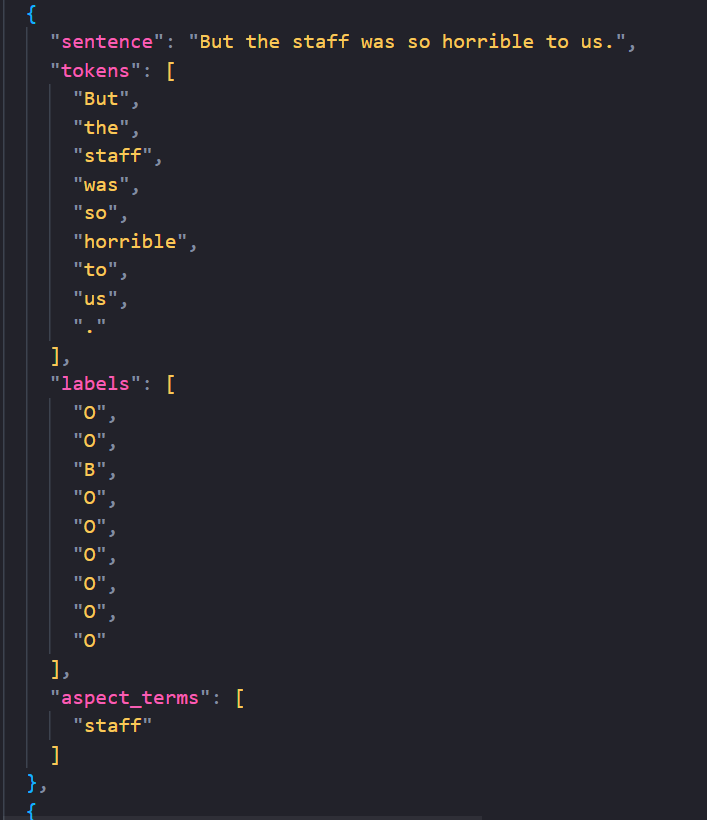
\includegraphics[width=0.5\linewidth]{image5.png}
    \caption{An instance from \texttt{train\_task\_1.json}}
\end{figure}

\subsection{Model Architectures \& Hyperparameters}
We experiment with two types of recurrent models (`RNN' and `GRU') using two pre-trained embedding sets (`GloVe' and `fastText'). All models use pre-trained embeddings directly (i.e., no custom vocabulary is built). The main architecture is as follows:
\begin{itemize}
    \item \textbf{Input:} Pre-trained word embeddings (300-dimensional) obtained from either GloVe or fastText.
    \item \textbf{Recurrent Layers:} A two-layer RNN/GRU is used. In our final implementation, the recurrent layers are non-bidirectional. (Bidirectional variants could further improve aspect span detection.)
    \item \textbf{Regularization:} A dropout layer with a probability of 0.3 is applied to the output of the recurrent layer to prevent overfitting.
    \item \textbf{Fully Connected Layer:} A linear layer maps the hidden representations to the output space corresponding to the BIO tags (with a label mapping: \texttt{\{<PAD>:0, O:1, B:2, I:3\}}).
    \item \textbf{Hyperparameters:}
    \begin{itemize}
        \item \textbf{Embedding Dimension:} 300 (fixed by the pre-trained embeddings).
        \item \textbf{Hidden Dimension:} 512.
        \item \textbf{Number of Layers:} 2.
        \item \textbf{Dropout:} 0.3.
        \item \textbf{Optimizer:} AdamW with a learning rate of 0.0005 and weight decay of $1 \times 10^{-4}$.
        \item \textbf{Scheduler:} We use a \texttt{ReduceLROnPlateau} scheduler that monitors the validation F1 score (mode=`max`) with a patience of 2 epochs.
    \end{itemize}
\end{itemize}

\subsection{Loss Plots}
The following figures show example loss curves for the models:
\begin{figure}[H]
    \centering
    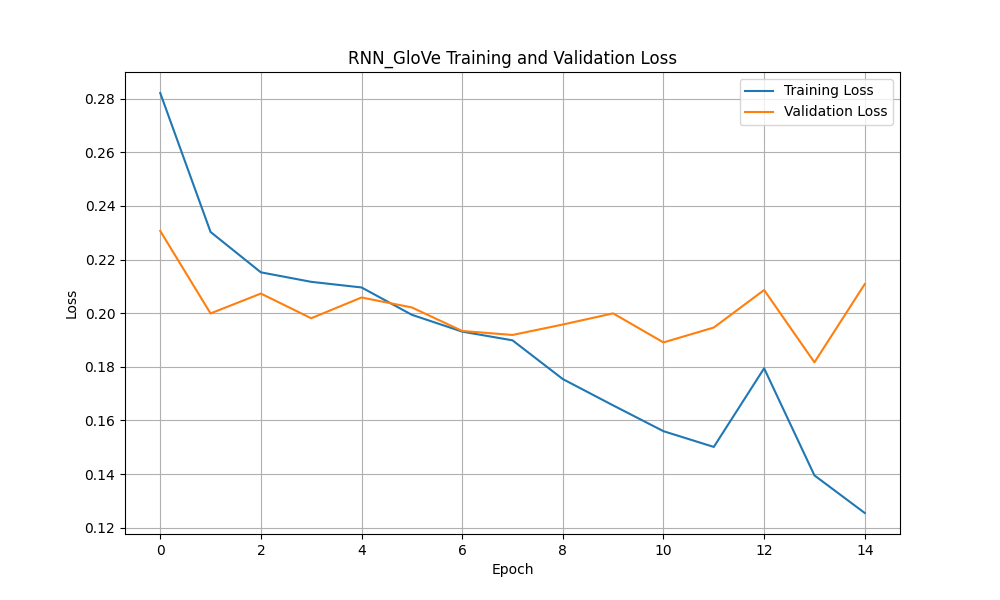
\includegraphics[width=0.5\linewidth]{image1.png}
    \caption{RNN with GloVe}
\end{figure}
\begin{figure}[H]
    \centering
    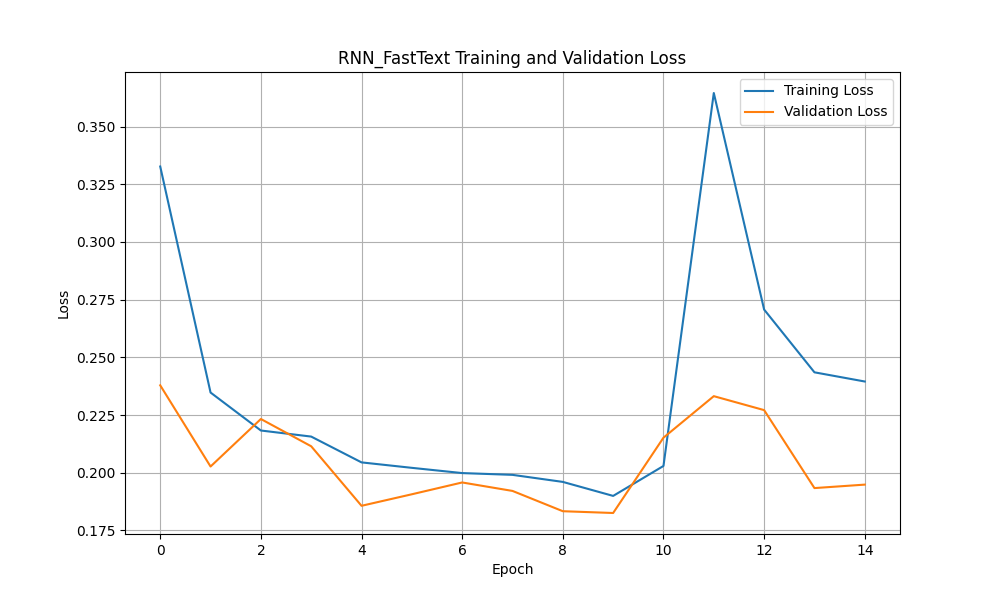
\includegraphics[width=0.5\linewidth]{image2.png}
    \caption{RNN with FastText}
\end{figure}
\begin{figure}[H]
    \centering
    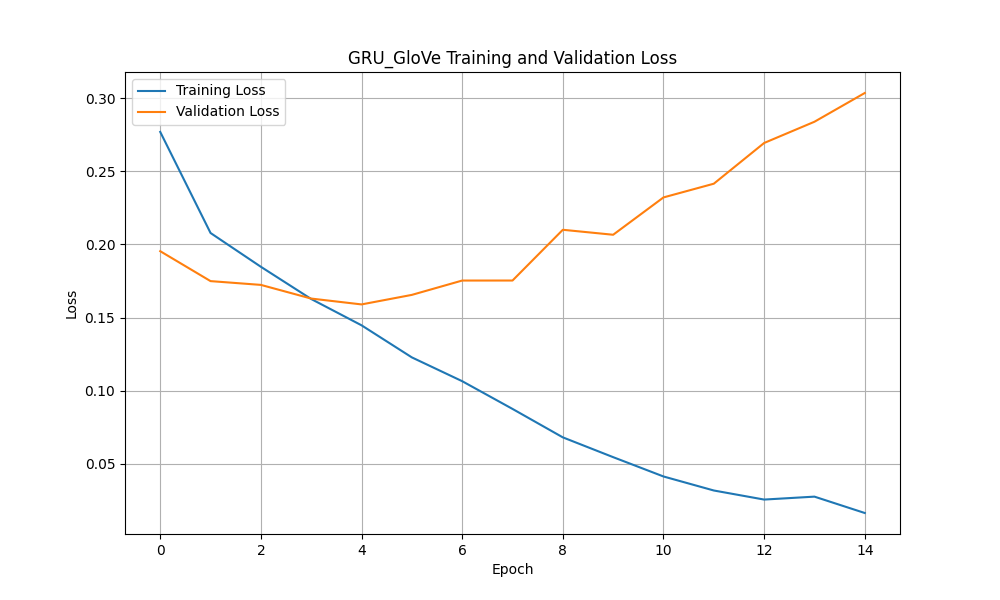
\includegraphics[width=0.5\linewidth]{image3.png}
    \caption{GRU with GloVe}
\end{figure}
\begin{figure}[H]
    \centering
    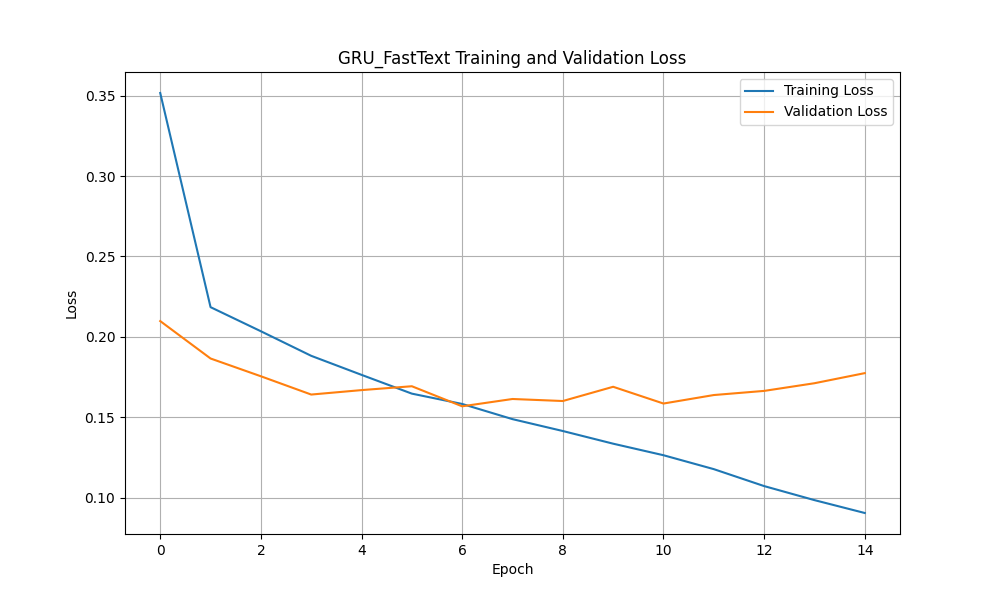
\includegraphics[width=0.5\linewidth]{image4.png}
    \caption{GRU with FastText}
\end{figure}

\subsection{Performance Comparison}
We trained four models:
\begin{itemize}
    \item RNN with GloVe embeddings
    \item RNN with fastText embeddings
    \item GRU with GloVe embeddings
    \item GRU with fastText embeddings
\end{itemize}
Performance was measured at both the token level (tag-level F1) and at the span level (chunk-level F1) using the conlleval evaluation script. Our experimental results were as follows:
\begin{table}[H]
\centering
\begin{tabular}{lcc}
\hline
\textbf{Model} & \textbf{Chunk-level F1} & \textbf{Tag-level F1} \\ \hline
RNN-GloVe    & 60\%   & 93.78\% \\
RNN-fastText  & 60.56\%   & 93.84\% \\
GRU-GloVe    & 61.76\%   & 94.52\% \\
GRU-fastText  & 64.61\%   & 94.58\% \\ \hline
\end{tabular}
\caption{Performance comparison on the validation set.}
\label{tab:performance}
\end{table}
\vspace{0.2cm}

The high tag-level F1 indicates accurate token-level predictions; however, the chunk-level F1 is lower, reflecting challenges in correctly identifying entire aspect spans.\\
\\
The models' performance is influenced by the quality of the embeddings and the type of recurrent unit:
\begin{itemize}
    \item \textbf{Embeddings:} FastText embeddings outperform GloVe in our experiments, especially at the chunk level. This is likely because FastText learns representations at the subword level. It can capture morphological features and handle out-of-vocabulary or misspelled words better than GloVe, which treats each word as an atomic unit.
    \item \textbf{Recurrent Units:} The GRU-based models generally perform better than the RNN-based models. GRU cells include gating mechanisms (reset and update gates) that help mitigate the vanishing gradient problem, allowing them to capture long-range dependencies more effectively. This results in improved performance in identifying complete aspect spans.
\end{itemize}

Additionally, all models exhibit some degree of overfitting. Notably, the GRU model with GloVe embeddings overfits the most. This could be because:
\begin{itemize}
    \item GloVe embeddings, while effective at capturing global co-occurrence statistics, do not incorporate subword information. As a result, the model may rely more on memorizing training examples.
    \item The GRU architecture, with its additional gating mechanisms and higher representational capacity, might be more prone to overfitting when combined with fixed embeddings.
\end{itemize}

There were also cases where \texttt{GRU\_GloVe} performed slightly better than \texttt{GRU\_FastText}. However, the difference was not huge and GRU with GloVe still experienced more overfitting than GRU with FastText. 

\subsection{Best Performing Model \& Evaluation}
The best-performing model, based on chunk-level F1, was \textbf{GRU-FastText} with a chunk F1 of 64.61\% (and tag F1 of 94.58\%). 

\subsection{Reasons for Performance}
\begin{itemize}
    \item \textbf{FastText Embeddings:} FastText embeddings improve performance because they capture subword-level information. This allows the model to better represent rare words and morphological variations, which is crucial for accurately identifying aspect term boundaries.
    \item \textbf{GRU Recurrent Unit:} GRU outperforms the standard RNN because its gating mechanisms help in effectively capturing long-term dependencies. This leads to more robust predictions of aspect spans, as the model can better utilize context from earlier and later parts of the sentence.
    \item \textbf{Overfitting:} The validation loss does not decrease much throughout as compared to the train loss. This could be improved upon through better feature engineering, bi-directional model and more complex architectures (like Conditional Random Field), embeddings and epochs.
\end{itemize}



\section{Task 2}
\subsection{Preprocessing}
\subsubsection{tokenize\_sentence(sentence)}

The function \texttt{tokenize\_sentence(sentence)} takes a sentence as input and breaks it down into individual words, known as tokens.

\begin{enumerate}
    \item Remove all symbols: The function removes any character that is not a word character such as punctuation marks like commas, periods, exclamation points, etc.

    \item Splitting on whitespace: After removing the symbols, the sentence is split into words at spaces and returns a list of individual words.
\end{enumerate}

\subsubsection{preprocess\_data(data)}
This function preprocesses a dataset containing sentences, their corresponding aspect terms, and sentiment polarity. It tokenizes sentences, identifies aspect terms, and determines their positions within the sentence. Then it outputs is a structured dataset as suggested in the assignment.
\\
\newline
The function iterates over each entry in \texttt{data} and

\begin{enumerate}
\item Tokenizes sentence using \texttt{tokenize\_sentence()}, which removes punctuation and splits the sentence into words.

\item Then it identifies Aspect Term Position in the sentence by iterating through the tokenized sentence and checking whether the aspect term matches a sequence of words in the sentence. If a match is found, the starting index of the aspect term in the tokenized sentence is recorded.

\item Then it constructes the Processed Entry of the following form and stores it - 
\begin{itemize}
    \item \texttt{tokens}: The tokenized sentence.
    \item \texttt{polarity}: The sentiment polarity of the aspect term.
    \item \texttt{aspect\_term}: The tokenized aspect term.
    \item \texttt{index}: The position of the aspect term in the tokenized sentence.
\end{itemize}

\end{enumerate}

\subsubsection{ABSA Dataset (Aspect Based Sentiment Analysis Dataset)}

The \texttt{ABSADataset} class extends the \texttt{Dataset} class from PyTorch and handles tokenization, encoding, and the preparation of necessary input features for the model.

\begin{enumerate}

\item Initializes - 
    \begin{itemize}
    \item \texttt{data}: A list of dictionary entries containing preprocessed text data.
    \item \texttt{tokenizer}: A tokenizer (such as BERT or another transformer model tokenizer) to encode sentences.
    \item \texttt{max\_len}: The maximum sequence length for tokenized inputs (default: 128).
\end{itemize}


\item The method \texttt{\_\_len\_\_} returns the total number of samples in the dataset.

\item The \texttt{\_\_getitem\_\_} method retrieves and processes a sample at a given index:
\begin{itemize}
    \item Extracts sentence tokens, aspect terms, aspect indices, and sentiment polarity.
    \item Ensures \texttt{aspect\_terms} and \texttt{aspect\_indices} are stored as lists.
    \item Converts sentiment polarity from textual labels (\texttt{negative, neutral, positive, conflict}) to numerical values using a mapping:
    \begin{verbatim}
    polarity_mapping = {'negative': 0, 'neutral': 1, 'positive': 2, 'conflict': 3}
    \end{verbatim}
    \item Tokenizes the sentence using the provided tokenizer, adding special tokens and ensuring the sequence is padded or truncated to the specified \texttt{max\_len}.
    \item Creates an \texttt{aspect\_mask}, a tensor marking the position of aspect terms in the sentence, accounting for the presence of special tokens - CLS at the beginning and SEP at the end.
\end{itemize}
\begin{center}
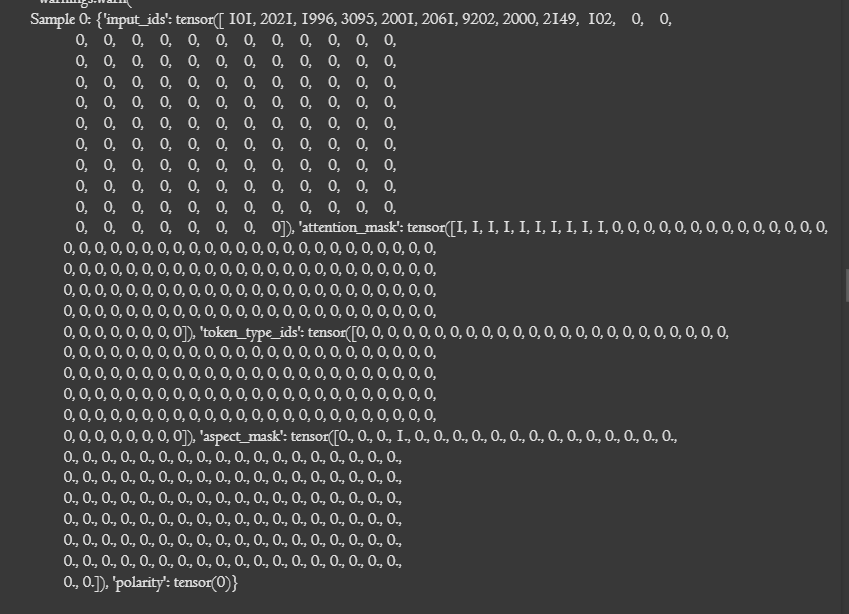
\includegraphics[width=1\textwidth]{ABSA Dataset.png}
\end{center}
\end{enumerate}

\subsection{Architectures}

\subsubsection{Model 1 - Interactive Multi Head Attention Network}
The first model that I tried used a combination of \textbf{BERT, Bidirectional GRU, Multi-Head Attention, and Aspect-Aware Position Embeddings}. 
\begin{itemize} 
\item BERT generated contextualized word embeddings, which are further refined using a \textbf{Bidirectional GRU (BiGRU)} to capture sequential dependencies. 
\item Aspect-aware \textbf{position embeddings} were added to enhance the model’s focus on aspect terms within a sentence. 
\item The model employs \textbf{two multi-head attention mechanisms}: (1) \textbf{Aspect-to-Context Attention}, where the aspect term learns from the context, and (2) \textbf{Context-to-Aspect Attention}, where the sentence learns relevant information from the aspect term. Then these attention outputs were concatenated and passed through a \textbf{fusion layer}.
\item The output layer then classified sentiment into different categories (e.g., positive, neutral, negative).
\end{itemize}
\begin{center}
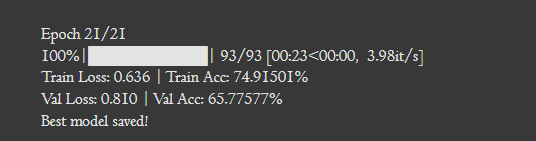
\includegraphics[width=0.75\textwidth]{Model_1_Accuracy.png}
\end{center}
\begin{center}
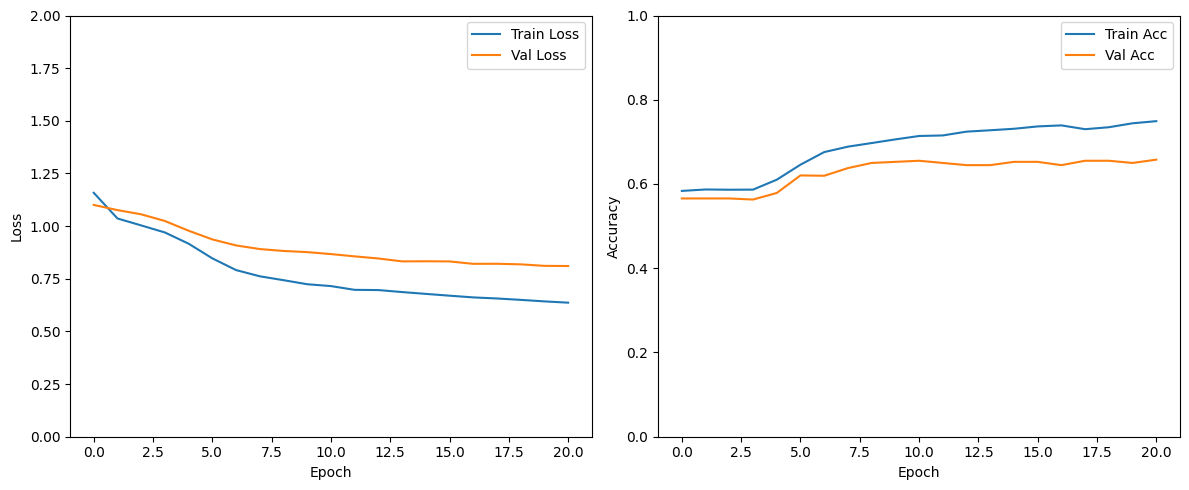
\includegraphics[width=1\textwidth]{Architecture 1.png}
\end{center}

\subsubsection{Model 2 - Graph-Based Sentiment Model }
The second model I tried was \textbf{Graph-Based Sentiment Model}. It first extracts \textbf{BERT embeddings} for contextualized word representations. These embeddings are refined using \textbf{Graph Convolutional Networks (GCN)}, which capture syntactic and semantic relationships through dependency-based adjacency matrices.

Next, a \textbf{Bidirectional LSTM (BiLSTM)} captures sequential dependencies, and an \textbf{attention mechanism} highlights the most relevant tokens. The outputs from \textbf{GCN and BiLSTM} are then fused via a \textbf{linear transformation layer}, combining syntactic and sequential knowledge. Finally, a \textbf{fully connected output layer} performs sentiment classification, effectively leveraging both structural and contextual information.
\begin{center}
\begin{center}
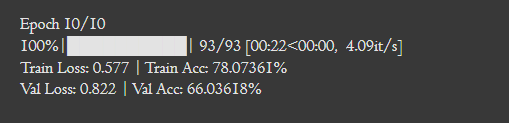
\includegraphics[width=0.75\textwidth]{Model_2_Accuracy.png}
\end{center}
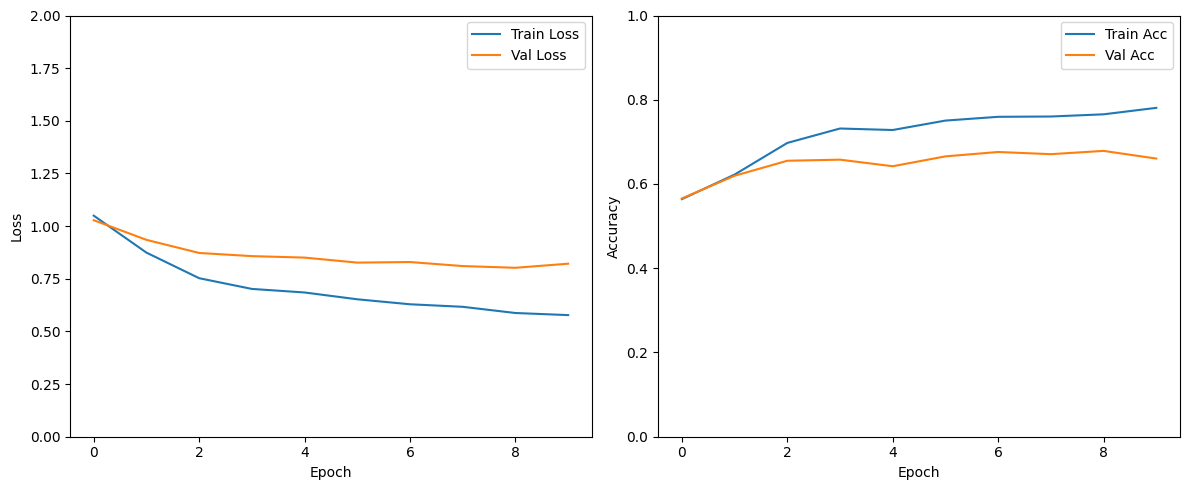
\includegraphics[width=1\textwidth]{Architecture 2.png}
\end{center}
\subsubsection{Model 3 - Target Dependent LSTM and GCN}

\paragraph{OVERVIEW}
The \textbf{TD\_LSTM\_GCN} model is designed for \textbf{aspect-based sentiment analysis (ABSA)} and incorporates three main components:
\begin{itemize}
    \item \textbf{BERT Encoder}: Extracts contextual embeddings from input text.
    \item \textbf{Target-Dependent LSTM (TD-LSTM)}: Captures the left and right contexts separately along with the aspect term.
    \item \textbf{Graph Convolutional Network (GCN)}: Uses dependency information to capture syntactic relationships.
    \item \textbf{Attention Fusion Mechanism}: Integrates TD-LSTM and GCN representations to enhance sentiment classification.
\end{itemize}


\paragraph{MODEL COMPONENTS}

\subparagraph{1. BERT Encoder}
\begin{itemize}
    \item The model initializes a \textbf{BERT-base} model (\texttt{bert-base-uncased}) to generate deep contextualized word embeddings.
    \item The \textbf{last hidden states} of BERT are used as input embeddings for subsequent modules.
\end{itemize}

\subparagraph{2. Target-Dependent LSTM (TD-LSTM)}
The TD-LSTM module consists of three LSTMs:
\begin{enumerate}
    \item \textbf{Left LSTM} ($lstm_{left}$): Processes words \textbf{before the aspect term}.
    \item \textbf{Right LSTM} ($lstm_{right}$): Processes words \textbf{after the aspect term}.
    \item \textbf{Target LSTM} ($lstm_{target}$): Processes the \textbf{aspect term itself}.
\end{enumerate}
Each LSTM is unidirectional, ensuring that the model processes left and right contexts separately to capture sentiment dependencies.

\subparagraph{3. Graph Convolutional Layer (GCN Implementation)}
\begin{itemize}
    \item \textbf{Adjacency Matrix Processing:}Self-loops are added to the adjacency matrix and the  matrix is normalized ($D^{-1/2} A D^{-1/2}$) for stability.
    \item \textbf{Feature Transformation:} The input is multiplied with a \textbf{learnable weight matrix}. The adjacency matrix is used to aggregate neighboring word features.

\end{itemize}
\subparagraph{4. Graph Convolutional Network (GCN)}
\begin{itemize}
    \item The model uses \textbf{multiple GCN layers} ($num\_gcn\_layers=2$) to capture syntactic dependencies between words.
    \item The input to GCN layers is the BERT embedding matrix.
    \item The adjacency matrix ($dependency\_matrix$) defines word relationships.
    \item Each GCN layer applies \textbf{graph convolution} followed by a ReLU activation.
\end{itemize}

\subparagraph{5. Attention Mechanism}
Two attention scores are computed:
\begin{enumerate}
    \item \textbf{LSTM-based attention}: Determines the importance of TD-LSTM features.
    \item \textbf{GCN-based attention}: Determines the importance of GCN features.
\end{enumerate}
The final representation is a \textbf{weighted sum} of TD-LSTM and GCN outputs, ensuring optimal feature integration.

\subparagraph{6. Fully Connected Layer (Classification Head)}: The final representation is concatenated ($hidden\_dim \times 3$) and passed through a \textbf{fully connected layer ($fc$)}. It produces sentiment classification output ($output\_dim=4$).

\paragraph{FORWARD PASS}

\begin{enumerate}
    \item \textbf{Input Processing:}$input\_ids$, $attention\_mask$, and $token\_type\_ids$ are fed into \textbf{BERT} to obtain contextual embeddings.
    \item \textbf{Dependency Matrix:} If no dependency matrix is provided, a simple heuristic-based approximation is created.
    \item \textbf{Aspect Term Identification:}The model identifies the start and end positions of aspect terms using $aspect\_mask$.
    \item \textbf{TD-LSTM Processing:}The \textbf{left}, \textbf{right}, and \textbf{target} representations are extracted using LSTMs.
    \item \textbf{Graph Convolution Processing:}
     The word embeddings pass through \textbf{GCN layers} to refine representations using syntactic dependencies. Aspect-specific representations are extracted from the GCN outputs.

    \item \textbf{Attention-Based Fusion:} Computes \textbf{importance scores} for TD-LSTM and GCN representations. Produces a \textbf{final hidden representation} using a weighted sum.
    \item \textbf{Classification:} The final representation is passed through a \textbf{fully connected layer} for sentiment prediction.
\end{enumerate}
\begin{center}
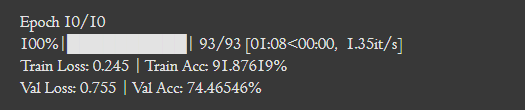
\includegraphics[width=0.75\textwidth]{Model_3_Accuracy.png}
\end{center}
\begin{center}
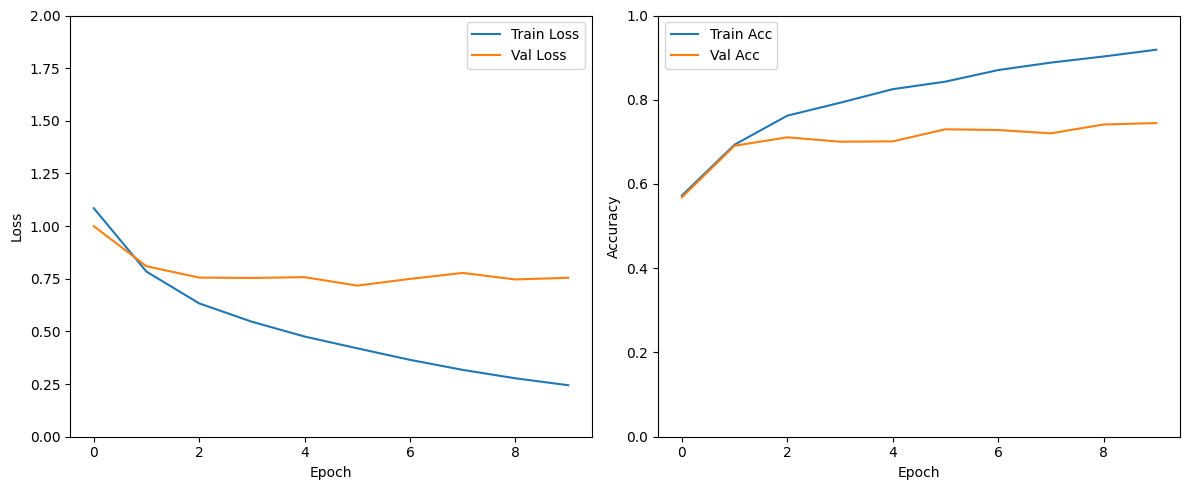
\includegraphics[width=1\textwidth]{Architecture 3.png}
\end{center}
\subsubsection{Hyperparameters Used}
\begin{itemize}
    \item Batch Size = 32
\item Output Dimension = 4
\item Maximum Sequence Lenght = 128
\item Hidden Dimension  256
\item Number of GCN Layers = 3
\item Learning Rate = 4e-6
\item Number of epochs = 10
\end{itemize}
Batch Size = 32
Output Dimension == 4
Maximum Sequence Lenght = 128
Hidden Dimension  256
Number of GCN Layers = 3
Learning Rate = 4e-6
Number of epochs = 10
\subsubsection{Justification of the Best Model - TD LSTM and GCN}
\begin{itemize}

    \item \textbf{Aspect-Specific Context Modeling}: Separately captures left, right, and aspect-specific dependencies for improved ABSA.

    \item \textbf{Enhanced Structural \& Contextual Understanding}: Combines sequential (TD-LSTM) and syntactic (GCN) modeling for richer sentiment representation.

    \item \textbf{Target-Specific Representations}: Prevents irrelevant aspect mixing by processing left and right contexts separately.

    \item \textbf{GCN for Dependency Parsing}: Incorporates syntactic relationships, making the model more robust to complex sentence structures.

    \item \textbf{Attention Fusion}: Selectively integrates crucial features from TD-LSTM and GCN for optimal classification.
    \item \textbf{Aspect-Specific Focus}: Explicitly processes aspect terms, ensuring sentiment analysis remains target-focused.

\end{itemize}

\subsection{Fine Tuning BERT, BART, RoBERTa - Additional Task}

\subsubsection{BERT for ABSA}
The \texttt{BERTForABSA} class fine-tunes BERT for ABSA by leveraging both the aspect representation and the sentence representation. The architecture consists of:
\begin{itemize}
    \item A BERT model pre-trained on general language understanding tasks.
    \item A dropout layer with a probability of 0.1 to prevent overfitting.
    \item A linear classifier that takes a concatenation of the aspect representation and the sentence representation.
\end{itemize}

The forward pass includes:
\begin{enumerate}
    \item Extracting contextualized token representations using BERT.
    \item Computing the aspect representation as the weighted sum of token embeddings, using an aspect mask.
    \item Extracting the sentence representation from the \texttt{[CLS]} token.
    \item Concatenating both representations and passing them through a classifier.
\end{enumerate}

\begin{center}
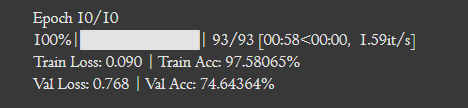
\includegraphics[width=0.75\textwidth]{Bert_Accuracy.png}
\end{center}
\begin{center}
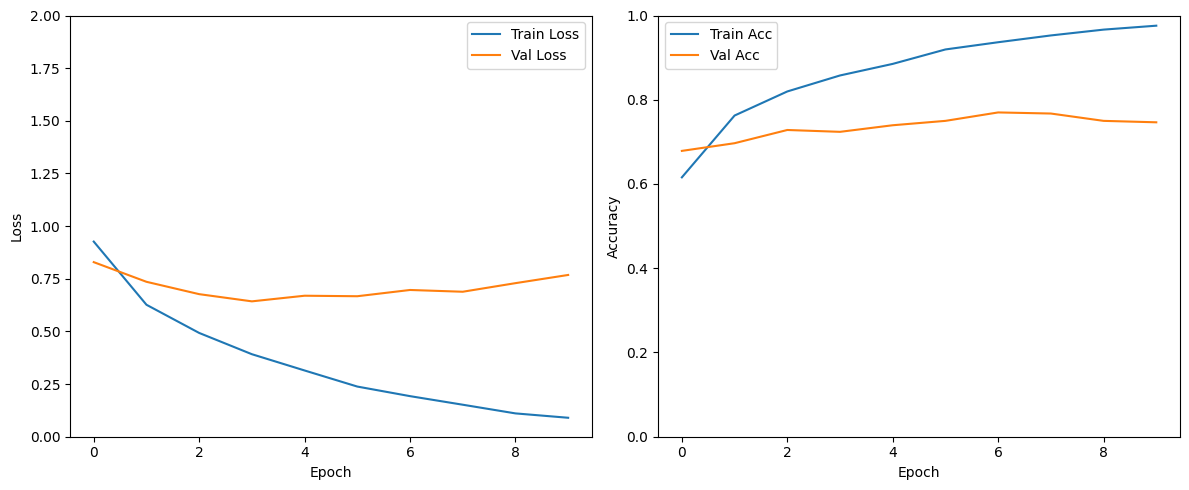
\includegraphics[width=1\textwidth]{Bert.png}
\end{center}
\subsubsection{BART for ABSA}
The \texttt{BARTForABSA} class is similar to the BERT model but uses BART, a denoising autoencoder-based model. Key characteristics include:
\begin{itemize}
    \item BART model as the feature extractor.
    \item A dropout layer with a probability of 0.1.
    \item A classifier that combines the aspect representation and sentence representation.
\end{itemize}
The architecture follows the same approach as BERT and RoBERTa, where:
\begin{enumerate}
    \item The model extracts contextual embeddings.
    \item Aspect and sentence representations are computed.
    \item These representations are concatenated and passed through a classifier.
\end{enumerate}

Differences from BERT:
\begin{itemize}
    \item BART does not use token type embeddings.
    \item Uses the first token's embedding for the sentence representation.
\end{itemize}
\begin{center}
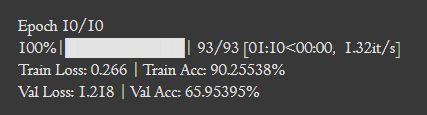
\includegraphics[width=0.75\textwidth]{Bart_Accuracy.png}
\end{center}
\begin{center}
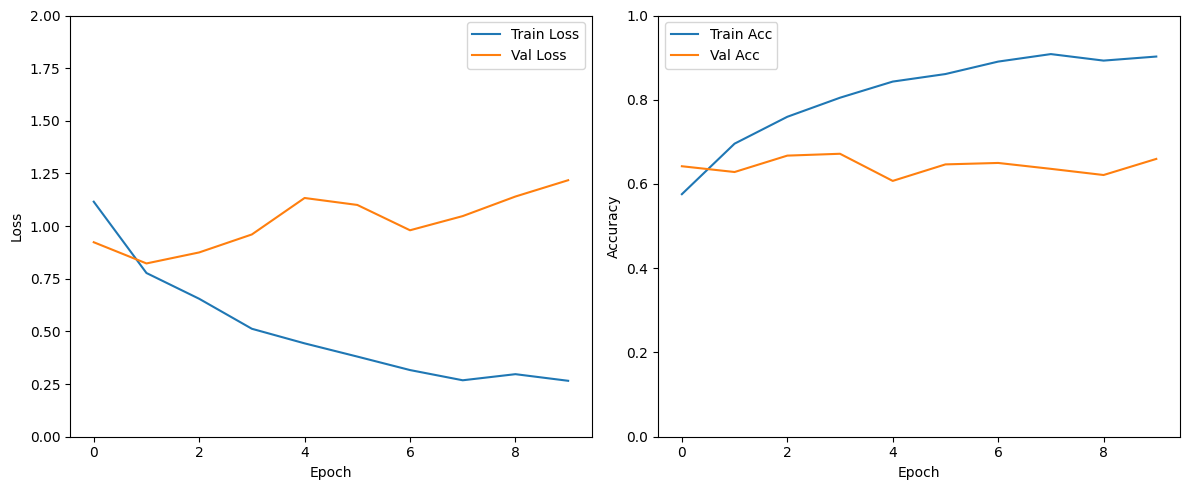
\includegraphics[width=1\textwidth]{Bart.png}
\end{center}


\subsubsection{RoBERTa for ABSA}
The \texttt{RoBERTaForABSA} class fine-tunes RoBERTa for ABSA. The architecture follows the same approach as BERT and BART, where:
\begin{enumerate}
    \item The RoBERTa model extracts contextual embeddings.
    \item Aspect and sentence representations are computed.
    \item These representations are concatenated and passed through a classifier.
\end{enumerate}

\begin{center}
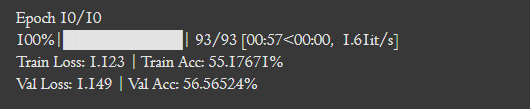
\includegraphics[width=0.75\textwidth]{Roberta_Accuracy.png}
\end{center}
\begin{center}
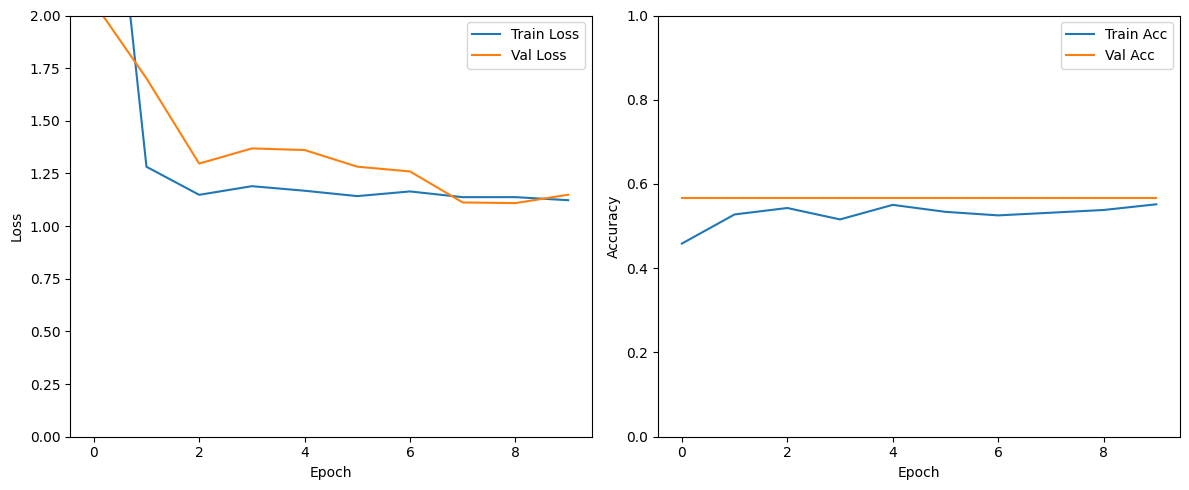
\includegraphics[width=1\textwidth]{Roberta.png}
\end{center}

\subsubsection{COMPREHENSIVE ANALYSIS}
\textbf{Why Does BERT Perform Best?}
\begin{itemize}
    \item \textbf{Bidirectional Context Encoding}: BERT’s Masked Language Model (MLM) + Next Sentence Prediction (NSP) training helps capture aspect-sentiment relationships effectively.
    \item \textbf{Token Type Embeddings}: Helps differentiate aspect terms from the sentence, improving classification.
    \item \textbf{Strong Sentence Representation}: Uses the \texttt{[CLS]} token, leading to better sentiment predictions.
\end{itemize}

\textbf{Why Does BART Underperform?}
\begin{itemize}
    \item Uses a \textbf{denoising autoencoder} for pretraining, which is less effective for fine-grained ABSA.
    \item \textbf{No token type embeddings}, making aspect-sentiment differentiation harder.
    \item \textbf{First token used for sentence representation}, which is weaker than BERT’s \texttt{[CLS]} token.
\end{itemize}

\textbf{Why Does RoBERTa Perform the Worst?}
\begin{itemize}
    \item \textbf{No token type embeddings} (like BART).
    \item \textbf{No NSP training}, reducing its ability to learn aspect-sentiment separation.
    \item \textbf{Aggressive pretraining on large data} helps general NLP tasks but not ABSA.
\end{itemize}

\section{Task 3}

\subsection{Dataset description and preprocessing}
The SQuADv2 dataset is used for the Question Answering task and has 130k samples in the training set and 12k samples in the validation set. The columns are id, title, context, question and answer. It has over 50k unanswerable questions, and it expects the model to abstain from answering if the question can not be answered from the given context.
\\
First, we convert the text input into tokens using the BERT tokenizer. We pass the question and context and get the tokenized output, where they are separated by [SEP] token and the it begins with [CLS] token. Since SpanBERT is an encoder-only model, it cannot give the answer in text format directly, so we predict the span of the answer and for that we need to find the answer in terms of token indices for fine-tuning and prediction tasks. Therefore, we store the start position and end positions in the preprocessing.

\subsection{Justification of model choices and hyperparameters}
I am using a subset of 60k samples for fine-tuning the models.
\\
SpanBERT: There were no changes with the architecture of SpanBERT. I tried 4 different configurations and the model was usually overfitting after the 2nd epoch. The best EM score was achieved with this configurations, so the hyperparameters are chosen empirically.
\\
SpanBERT-CRF: I have added two CRF layers, one for each start position and end position. I have also added extra hidden layers between the CRF layers and the final hidden layer of SpanBERT, so it can learn better representations. For this model as well, the hyperparameters were chosen empirically when the best EM score was achieved.

\subsection{Training and validation plots}
\begin{center}
    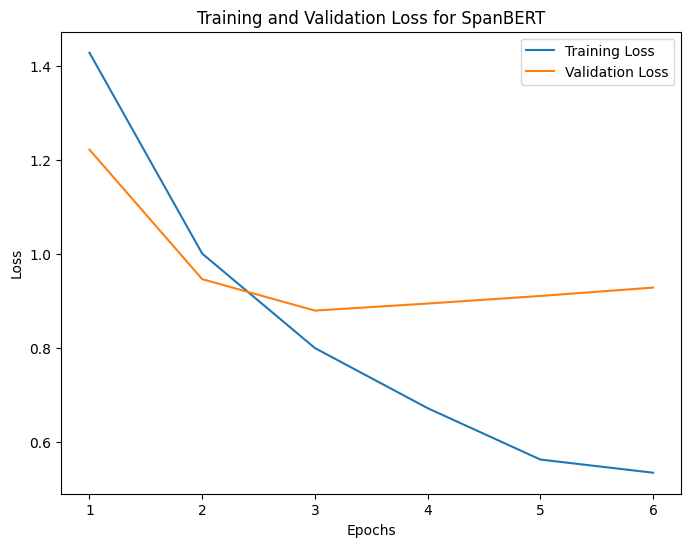
\includegraphics[width=0.55\textwidth]{spanbert_loss.png}
\end{center}
\begin{center}
    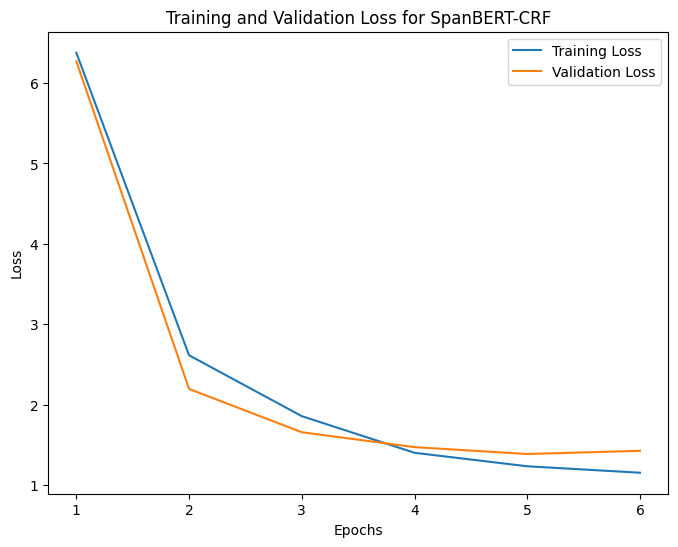
\includegraphics[width=0.55\textwidth]{crf_loss.png}
\end{center}

\subsection{Comparative analysis of SpanBERT-CRF and SpanBERT}
The SpanBERT model tends to overfit after 3rd epoch whereas the SpanBERT-CRF model slightly overfits after 5th epoch. SpanBERT model has lower values for loss on both training and validation sets. Even though SpanBERT overfits earlier, it has a better exact match score on the validation set than SpanBERT-CRF.

\subsection{Exact-match scores on the validation set}
\begin{center}
    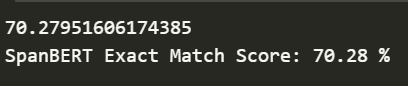
\includegraphics[width=0.55\textwidth]{spanbert_em.png}
\end{center}
\begin{center}
    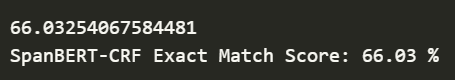
\includegraphics[width=0.55\textwidth]{crf_em.png}
\end{center}

\section{Individual Contribution}
\begin{itemize}
    \item Himanshu Raj: Task 3 implementation and report
    \item Ishita: Task 2 implementation and report
    \item Ritika Thakur: Task 1 implementation and report
\end{itemize}

\section{References}
\begin{itemize}
    \item \href{https://github.com/sighsmile/conlleval}{https://github.com/sighsmile/conlleval}
    \item \href{https://nlp.stanford.edu/projects/glove/}{https://nlp.stanford.edu/projects/glove/}
    \item \href{https://fasttext.cc/docs/en/english-vectors.html}{https://fasttext.cc/docs/en/english-vectors.html}
    \item \href{https://github.com/TarikBugraAy/BERT_Fine_Tune_For_ABSA}{https://github.com/TarikBugraAy/BERT\_Fine\_Tune\_For\_ABSA}
    \item \href{https://huggingface.co/learn/nlp-course/en/chapter7/7}{https://huggingface.co/learn/nlp-course/en/chapter7/7}
    \item \href{https://github.com/huggingface/transformers/blob/main/src/transformers/models/bert/modeling_bert.py}{https://github.com/huggingface/transformers/blob/main/src/transformers/models/bert/modeling_bert.py }
\end{itemize}

\end{document}